
\documentclass[xcolor={dvipsnames}]{beamer}
\usepackage{amsmath,amsfonts,amssymb,pxfonts,eulervm,xspace}
\usepackage{graphicx}
\usepackage{tikz}
 \usepackage{multimedia}
\usepackage{media9}
\usepackage{minted}
\usepackage{mathtools}

\usepackage{animate}

\graphicspath{{./figures/}}
\usetheme{ccnycrest}


\begin{document}

\title{ CS102: Inheritence}
\author{Hannah Aizenman}
\date{haizenm00@ccny.cuny.edu}


\begin{frame}
	\titlepage
\end{frame}

\begin{frame}{Shape: Triangle}
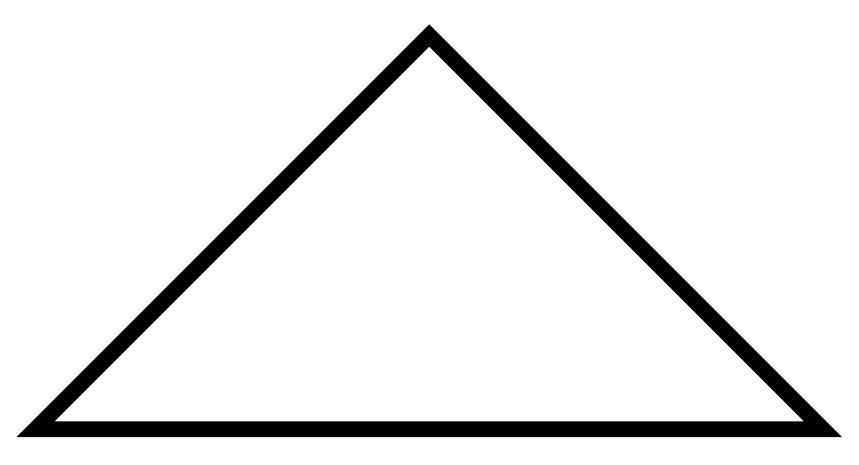
\begin{tikzpicture}[line width=2mm]
	\draw (5,5)--(10,0)--(0,0)--(5,5)--(10,0);
\end{tikzpicture}
\end{frame}

\begin{frame}[fragile]{Triangle Class}
\begin{minted}{c++}
class Triangle{
    private:
        static const int NSIDES=3;
        Point verts[NSIDES];
    public:
        Triangle(Point p1n, Point p2n, Point p3n);
        double perimeter();
        double area();
}
\end{minted}
\end{frame}


\begin{frame}{Shape: Square}
\begin{center}
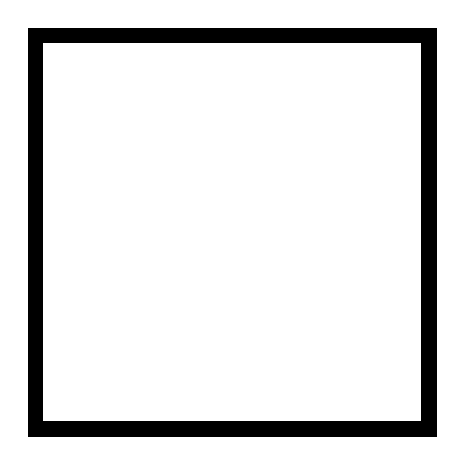
\begin{tikzpicture}[line width=2mm]
	\draw (0,0)--(0,5)--(5,5)--(5,0)--(0,0)--(0,5);
\end{tikzpicture}
\end{center}
\end{frame}

\begin{frame}[fragile]{Square Class}
\begin{minted}{c++}
class Square{
    private:
        static const int NSIDES=4;
        Point verts[NSIDES]
    public:
        Square(Point p1n, Point p2n, Point p3n, Point p4n);
        double perimeter();
        double area();
}
\end{minted}
\end{frame}

\begin{frame}[fragile]{Perimeter functions} 
\begin{block}{Triangle}
\begin{minted}{c++}
double Triangle::perimeter(){
    return distance(verts[0], verts[1]) + 
           distance(verts[1], verts[2]) + 
           distance(verts[2], verts[0]);
}
\end{minted}
\end{block}
\pause
\begin{block}{Square}
\begin{minted}{c++}
double Square::perimeter(){
    return distance(verts[0], verts[1]) + 
           distance(verts[1], verts[2]) + 
           distance(verts[2], verts[3]) +
           distance(verts[3], verts[0]);
}
\end{minted}
\end{block}
\end{frame}

\begin{frame}[fragile]{Base: Shape}
\begin{minted}{c++}
class Shape{
    protected:
        static const int NSIDES = 1;
        Point verts[NSIDES];
    public:
        double perimeter();
        double area();
};
\end{minted}
\end{frame}

\begin{frame}[fragile]{Generic Perimeter}
\begin{minted}{c++}
double Shape::perimeter(){
    double perim=0;
    for (int i=0; i<NSIDES-1; i++){
        perim+=distance(verts[i], verts[i+1]);
    }
        
    perim+=distance(verts[NSIDES-1],verts[0]);
    return perim;
}
\end{minted}
\end{frame}

\begin{frame}[fragile]{Derived: Triangle}
\begin{minted}{c++}
class Triangle : public Shape {
    private:
        static const int NSIDES=3;
    public:
        Triangle(Point p1n, Point p2n, Point p3n);
        double area();
};
\end{minted}
\end{frame}

\begin{frame}[fragile]{Derived: Square}
\begin{minted}{c++}
class Square : public Shape {
    private:
        static const int NSIDES=4;
    public:
        Square(Point p1n, Point p2n, Point p3n, Point p4n);
        double area();
};
\end{minted}
\end{frame}

\begin{frame}{Member and Method Access Rules}
	\begin{block}{Inherited Access Restrictions}
	\begin{center}
	\begin{tabular}{l|l|l|l}
		  & \textbf{Public} & \textbf{Protected} & \textbf{Private}\\\hline
		\textbf{Same Class} & yes & yes & yes\\
		\textbf{Derived Class} & yes & yes & no\\
		\textbf{Outside Class} & yes & no & no\\
	\end{tabular}
	\end{center}
	\end{block}
\pause
\begin{block}{Derived Classes \textbf{don't} inherit:}
	\begin{itemize}
		\item Constructors, destructors and copy constructors
		\item Overloaded operators
		\item Friend functions
	\end{itemize}
\end{block}
\end{frame}
\end{document}
